\documentclass[letterpaper,12pt,notitlepage,twoside]{report}

\newcommand{\watermark}{hello there}
\newcommand{\booktopic}{Machine Learning Operations}
\newcommand{\lastname}{Okoli}
\usepackage{NoteStyle}
\usepackage{placeins}
\usepackage{listings}

\definecolor{codegreen}{rgb}{0,0.6,0}
\definecolor{codegray}{rgb}{0.5,0.5,0.5}
\definecolor{codepurple}{rgb}{0.58,0,0.82}
\definecolor{backcolour}{rgb}{0.95,0.95,0.92}

\lstdefinestyle{mystyle}{
    backgroundcolor=\color{backcolour},   
    commentstyle=\color{codegreen},
    keywordstyle=\color{magenta},
    numberstyle=\tiny\color{codegray},
    stringstyle=\color{codepurple},
    basicstyle=\ttfamily\footnotesize,
    breakatwhitespace=false,         
    breaklines=true,                 
    captionpos=b,                    
    keepspaces=true,                 
    numbers=left,                    
    numbersep=5pt,                  
    showspaces=false,                
    showstringspaces=false,
    showtabs=false,                  
    tabsize=2
}

\lstset{style=mystyle}

\title{Machine Learning Operations}
\author{Chuks Okoli}
\date{\footnotesize Last Updated: \today}

\hypersetup{
  pdftitle={Machine Learning Operations},
  pdfauthor={Chuks Okoli},
  pdfsubject={},
}

% ToC on the title page:
% https://tex.stackexchange.com/a/45863
\makeatletter
\newcommand*{\toccontents}{\@starttoc{toc}}
\makeatother

\begin{document}

\begin{titlepage}
  \pagestyle{plain}
  \maketitle
  \setcounter{tocdepth}{2}

  \pdfbookmark[section]{\contentsname}{toc}
  \toccontents
  % Separate page:
  % \tableofcontents
\end{titlepage}

\chapter{Introduction} \label{ch:1}
\inspiration{Imagine you have a magic cookbook that can teach you how to make the best cookies ever. But it's not just any cookbook, it's a special one that learns and gets better every time you make cookies.

Now, making cookies is a bit like solving a puzzle. You need the right ingredients (like flour, sugar, and chocolate chips) and you need to mix them together in just the right way. Sometimes, you might make a mistake and your cookies don't turn out quite right.

That's where MLOps comes in! MLOps is like having a team of helpful fairies who watch over you while you're baking. They make sure you're using the right ingredients, they help you mix everything together perfectly, and they even give you tips on how to make your cookies even better next time.

So, with MLOps, you can keep making cookies and your magic cookbook will keep learning from each batch. And before you know it, you'll be making the most delicious cookies anyone has ever tasted!}{Chuks Okoli}{}

\firstletter{Hello there}, and welcome to \booktopic. This work is a culmination of hours of effort to create my reference for machine learning operations. All of the explanations are in my own words but majority of the content are based on Alexey Grigorev's DataTalksClub \href{https://github.com/DataTalksClub/mlops-zoomcamp}{MLOps Zoomcamp course}.

\section{What is MLOps?}
\inspiration{MLOps, also known as DevOps for machine learning, is an umbrella term that encompasses philosophies, practices, and technologies that are related to implementing machine learning lifecycles in a production environment.}{Microsoft Blog}{}

Machine Learning Operations (MLOps) is a set of best practices for putting machine learning models into production. The process for a machine learning project involves:
\begin{itemize}
	\item Design - define if machine learning is the right tool for solving the problem
	\item Train - train the model to find the best possible model
	\item Operate - deploy the model,  and monitor degradation or quality of the model
\end{itemize}
MLOps is a set of practices for automating everything and working together as a team on a machine learning project.

 \begin{funfact}[frametitle=\facttitlep{Fun Fact}{MLOps Principles}]
As machine learning and AI become more common in software, it's important to create guidelines and tools for testing, deploying, managing, and monitoring ML models in real-world use. This is where MLOps comes in. It helps prevent ``technical debt'' in machine learning projects by ensuring smooth operation and maintenance of models throughout their lifecycle.
\end{funfact}

MLOps helps to manage and orchestrate the end-to-end machine learning lifecycle by ensuring models are consistently accessible, reproducible, and scalable. It focuses on automating deployment and monitoring of ML pipelines while optimizing the model development process.

The three-phase approach to implementing machine learning (ML) solutions are:
\begin{itemize}
\item \textbf{Business Understanding and Design}: This phase involves identifying user needs, designing ML solutions to address them, and assessing project development. Prioritizing ML use cases and defining data requirements are key steps. The architecture of the ML application, serving strategy, and testing suite are designed based on functional and non-functional requirements.
\item \textbf{ML Experimentation and Development}: This phase focuses on verifying the applicability of ML by implementing Proof-of-Concept models. It involves iteratively refining ML algorithms, data engineering, and model engineering to deliver a stable, high-quality ML model for production.
\item \textbf{ML Operations}: Here, the emphasis is on deploying the developed ML model into production using established DevOps practices. Testing, versioning, continuous delivery, and monitoring are essential aspects of this phase.
\end{itemize}
These phases are interconnected, with design decisions influencing experimentation and deployment options.

\begin{figure}[h]
	\centering
	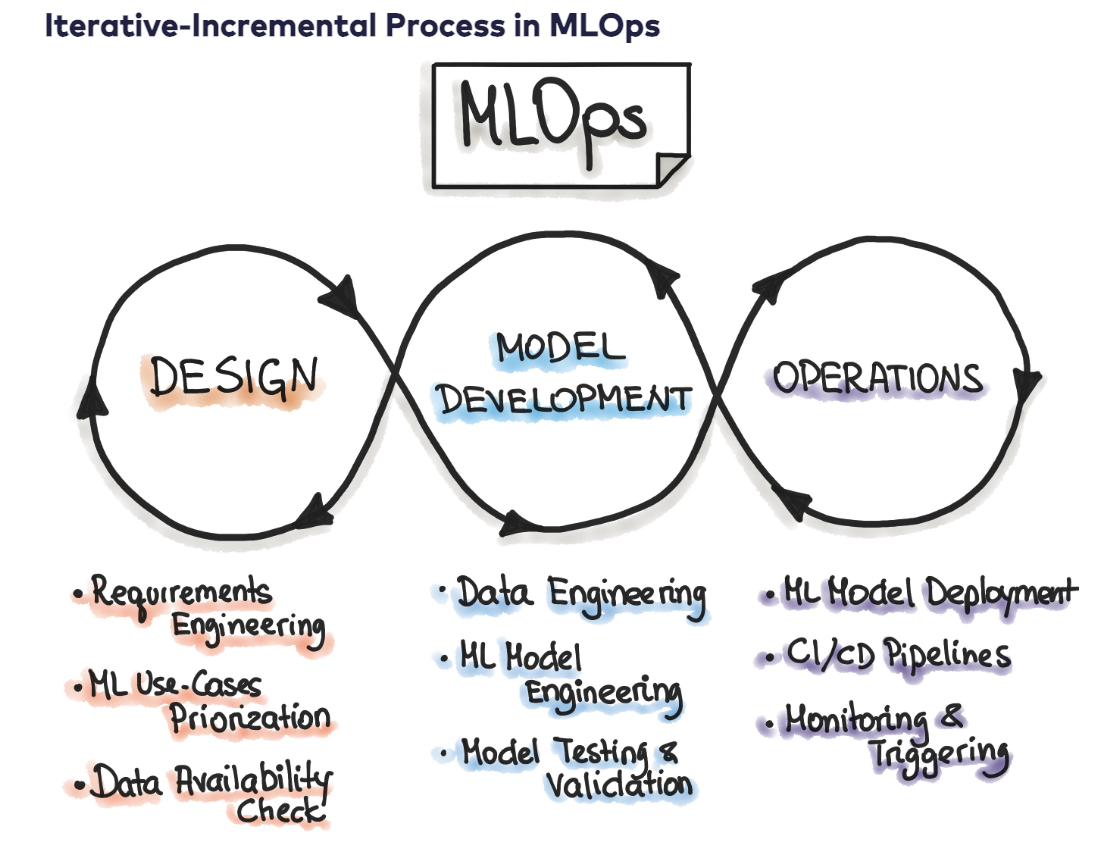
\includegraphics[width=\textwidth]{Images/Iterative MLOps.png}
	\caption{The complete MLOps process includes three broad phases of ``Designing the ML-powered application'', ``ML Experimentation and Development'',  and ``ML Operations''.}
	\label{fig:1}
\end{figure}
\FloatBarrier

MLOps leverages various tools to simplify the machine learning lifecycle.
\begin{itemize}[label={--}]
\item \textbf{Machine learning frameworks} like Kubernetes, TensorFlow and PyTorch for model development and training.
\item \textbf{Version control systems} like Git for code and model version tracking.
\item \textbf{CI/CD tools} such as Jenkins or GitLab CI/CD for automating model building, testing and deployment.
\item \textbf{MLOps platforms} like Kubeflow and MLflow manages model lifecycles, deployment and monitoring.
\item \textbf{Cloud computing platforms} like AWS, Azure and IBM Cloud provide scalable infrastructure for running and managing ML workloads.
\end{itemize}


\section{Environment Preparation}
\subsection{Configuring Environment with GitHub Codespaces}
To configure the environment using GitHub codespaces, first create a repository on GitHub, give the repository a name, add a ``README'' file and a \texttt{.gitignore} template, choose a license and create the repo. In the repo main page, click on \texttt{Create codespace on main} as shown in \textbf{Fig. \ref{fig:2}}.
\begin{figure}[h]
	\centering
	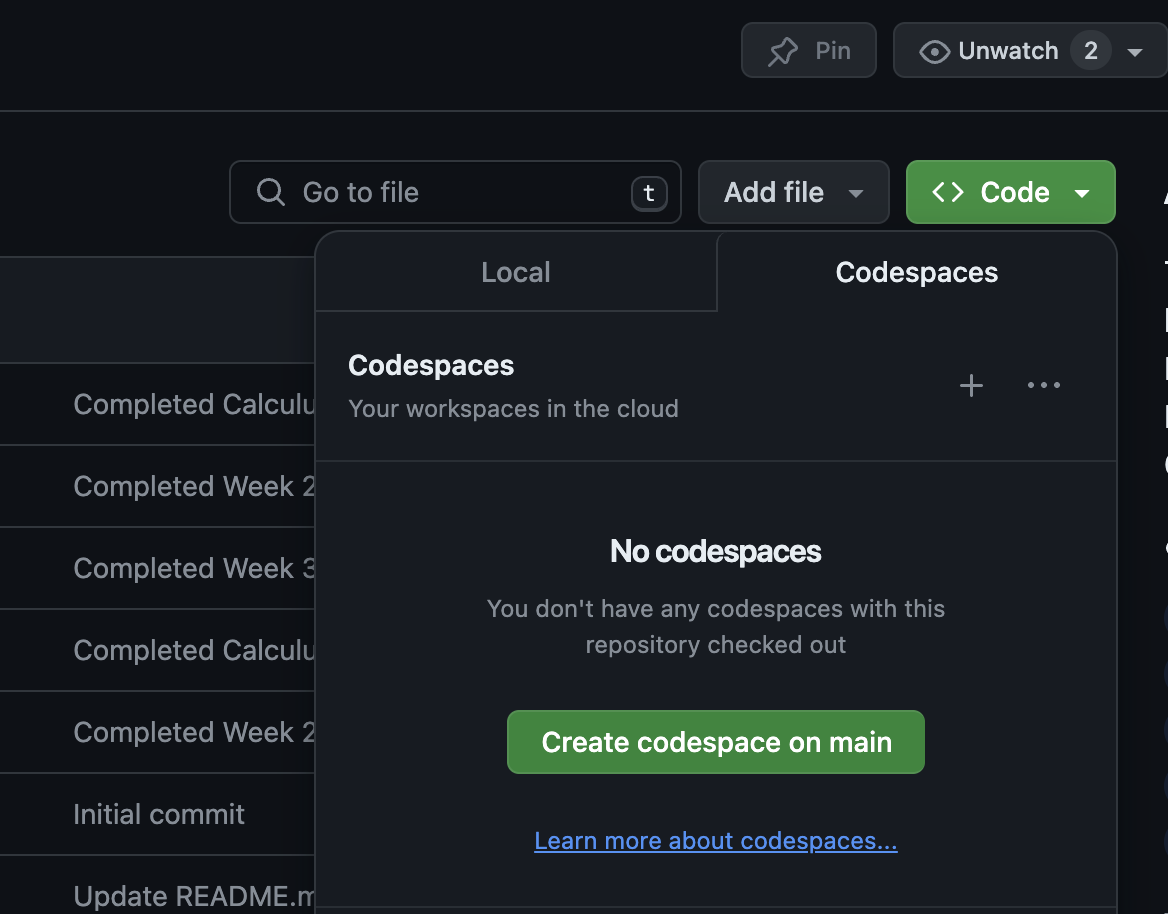
\includegraphics[width=0.5\textwidth]{Images/Codespaces.png}
	\caption{GitHub Codespaces setup}
	\label{fig:2}
\end{figure}
\FloatBarrier

A connection to Visual Studio Code can be made through Codespaces.  Start a new terminal, change directory to the workspaces and download and install Anaconda distribution of python in it using the step below.
 \begin{itemize}
\item \textbf{Step 1}: Download and install the Anaconda distribution of Python 
\begin{lstlisting}[language=python, numbers=none]
wget https://repo.anaconda.com/archive/Anaconda3-2022.05-Linux-x86_64.sh
\end{lstlisting}
\item \textbf{Step 2}: Run this command: 
\begin{lstlisting}[language=python, numbers=none]
bash Anaconda3-2022.05-Linux-x86_64.sh
\end{lstlisting}

After installing Anaconda, initialize it. In a new terminal, confirm that Anaconda is running in the workspaces
\begin{lstlisting}[language=python, numbers=none]
(base) @your_username -> /workspaces/mlops-zoomcamp-2024 (main) $ which python
/home/codespace/anaconda3/bin/python
\end{lstlisting}
\item \textbf{Step 3}: Make sure to install \texttt{pyarrow} in order to download parquet file
\begin{lstlisting}[language=python, numbers=none]
!pip install pyarrow
\end{lstlisting}
\item \textbf{Step 4}: Run jupyter notebook
\begin{lstlisting}[language=python, numbers=none]
jupyter notebook
\end{lstlisting}
\end{itemize}

\subsection{Configuring Environment with Amazon Web Service (AWS)}
To install using AWS,  create an account in AWS, go to EC2 and create an instance. Select the OS to use e.g. Ubuntu with 64-bit(x86) architecture. Select the instance type that will be sufficient for your project. Configure the cloud resources and launch. \\
Recommended development environment: Linux

 \begin{itemize}
\item \textbf{Step 1}: Download and install the Anaconda distribution of Python 
\begin{lstlisting}[language=python, numbers=none]
wget https://repo.anaconda.com/archive/Anaconda3-2022.05-Linux-x86_64.sh
bash Anaconda3-2022.05-Linux-x86_64.sh
\end{lstlisting}
\item \textbf{Step 2}: Update existing packages
\begin{lstlisting}[language=python, numbers=none]
sudo apt update
\end{lstlisting}
\item \textbf{Step 3}: Install Docker
\begin{lstlisting}[language=python, numbers=none]
sudo apt install docker.io
\end{lstlisting}
To run docker without sudo:
\begin{lstlisting}[language=python, numbers=none]
sudo groupadd docker
sudo usermod -aG docker \$USER
\end{lstlisting}
\item \textbf{Step 4}: Install Docker Compose
Install docker-compose in a separate directory
\begin{lstlisting}[language=python, numbers=none]
mkdir soft
cd soft
\end{lstlisting}
To get the latest release of Docker Compose, go to https://github.com/docker/compose and download the release for your OS.
\begin{lstlisting}[language=python, numbers=none]
wget https://github.com/docker/compose/releases/download/v2.5.0/docker-compose-linux-x86_64 -O docker-compose
\end{lstlisting}
Make it executable
\begin{lstlisting}[language=python, numbers=none]
chmod +x docker-compose
\end{lstlisting}
Add the soft directory to PATH. Open the .bashrc file with nano:
\begin{lstlisting}[language=python, numbers=none]
nano ~/.bashrc
\end{lstlisting}
In .bashrc, add the following line:
\begin{lstlisting}[language=python, numbers=none]
export PATH="${HOME}/soft:${PATH}"
\end{lstlisting}
Save it and run the following to make sure the changes are applied:
\begin{lstlisting}[language=python, numbers=none]
source ~/.bashrc
\end{lstlisting}
\item \textbf{Step 5}: Run Docker
\begin{lstlisting}[language=python, numbers=none]
docker run hello-world
\end{lstlisting}
\end{itemize}

\section{Model Development}
\subsection{Taxi trip prediction with machine learning}
    \begin{example}[frametitle=\extitle{Predict Taxi Trip}]
      This one will increment the counter automatically, resetting for each
      chapter.
    \end{example}


\section{On Colorful Boxes}
There are lots of different boxes you can make:
%
\begin{itemize}
  \item Like this one,
    \begin{notebox}
      which is wrapped in gray. I use it for notes.\ldots
    \end{notebox}

  \item Or this one,
    \begin{funfact}
      which is wrapped in red. I use it for fun facts or other asides\ldots
    \end{funfact}

  \item Or this one,
    \begin{mathaside}
      which is wrapped in blue and used for mathy stuff.
    \end{mathaside}

  \item Or this last one,
    \begin{example}
      which is wrapped in green. With a title, it's used for enumerated examples
      (see \smtt{\textbackslash extitle} and \smtt{\textbackslash excounter}).
      Observe:
    \end{example}

    \begin{example}[frametitle=\extitle{Test}]
      This is an example. What's the answer to $2+2$?
      \answer{Obviously 4, lol.}
    \end{example}

    \begin{example}[frametitle=\extitle{Test Again}]
      This one will increment the counter automatically, resetting for each
      chapter.
    \end{example}


  \item For red and blue boxes, there are custom commands for titles, too:
    \begin{mathaside}[frametitle=\mathtitle{One Title}]
      Like this
    \end{mathaside}
    \begin{mathaside}[frametitle=\mathtitlep{Two Titles}{A Subtitle}]
      Or this
    \end{mathaside}
\end{itemize}

\hr{5in}

These styles also automatically apply to theorems and claims.

\begin{theorem}[Pythagorean Theorem]
  \label{thm:pyth}
  For any right triangle with legs $a,b$ and hypotenuse $c$:
  %
  \begin{equation}
    \label{eq:pyth}
    a^2+b^2=c^2
  \end{equation}
\end{theorem}
\begin{proof}
  This is left as an exercise to the reader.
\end{proof}

\begin{claim}
  This is the greatest note template in the world.
\end{claim}

\hr{5in}

There are different ways to quote things, too, depending on how you want to
emphasize:

\begin{quoting}
  This is a simple, indented quote with small letters and italics usually
  suitable for in-text quotations when you just want a block.
\end{quoting}

Alternatively, you can use the \smtt{\textbackslash inspiration} command from
the chapter heading, which leverages the \smtt{thickleftborder} frame
internally, but adds a little more padding and styling (there's also just
\smtt{leftborder} for a thinner variant):

\begin{thickleftborder}
  Hello there!
\end{thickleftborder}



\section{On Cross-Referencing}
\marginnote{\footnotesize\softtext This is the standard way to include margin
notes. There are also commands to link to source papers directly (see
\smtt{\textbackslash lesson}).} You can reference most things---see
\autoref{thm:pyth} or \eqref{eq:pyth} or the \nameref{ch:1} chapter---directly
and easily as long as you give them labels. These are ``built-ins.'' However,
you can also create a \term{custom term} that will be included in the index,
then include references to it that link back to the original definition. Try
clicking: \refterm{custom term}. Building the index is on you, though. You can
also reference by using a different term for the text: \reftermx{custom
term}{like this}. Sometimes it doesn't fit the \termx{grammar}{grammatical
structure} of the sentence so you can define the term one way and visualize it
another way (this creates a \aterm{grammar} entry in the index). There's also
\prop{math terms} and a way to reference them: \refprop{math terms} (clickable),
but they do \textbf{not} show up in the index.



\section{On Math}
Most of the math stuff is just macros for specific things like the convolution
operator, $\conv$, probabilities, $\cprob{A}{B=C}$, or big-$O$ notation,
$\bigO{n^2\log{n}}$ but there's also a convenient way to include explanations on
the side of an equation:
%
\begin{align*}
  1 + 1 &\overset{?}{=} 2    \sideblock{2in}{first we do this} \\
      2 &\overset{?}{=} 2    \sideblock{2in}{then we do this} \\
      2 &= 2 \qed
\end{align*}

These are all in the \smtt{CustomCommands.sty} file.



\end{document}

